%
% Capítulo 3
%
\chapter{Solução do Problema} \label{cap3}

\section{Modelo de Dados}\label{sec31}

% Modelo EA
\subsection{Modelo Entidade-Associação}

\begin{figure}
	\centering
	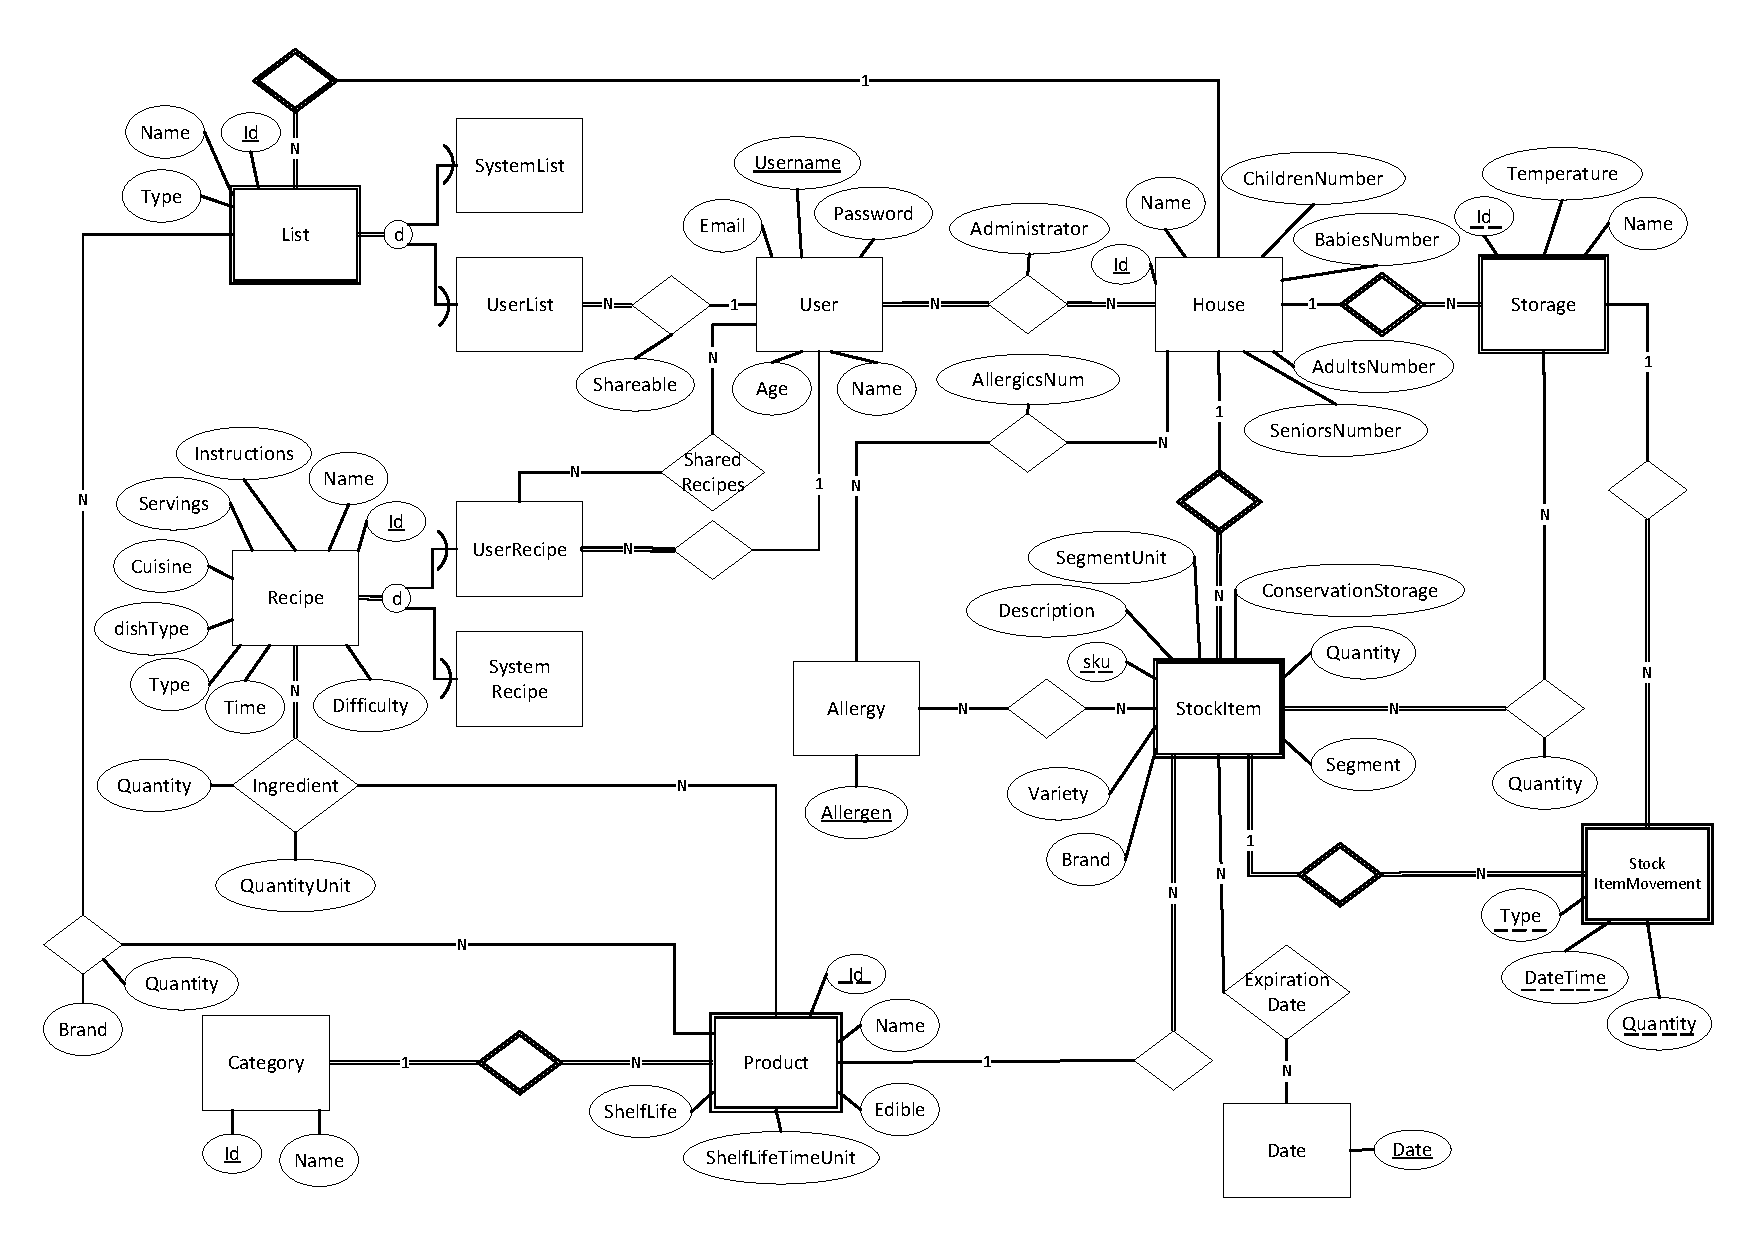
\includegraphics[width=20cm,height=16cm,scale=0.5]{./files/EA.pdf}
	\caption{Modelo Entidade-Associação}
	\label{modelo-ea}
\end{figure}

% Modelo Relacional
\subsection{Modelo Relacional}
{\parindent 0pt
	\begin{description}
		\item House(house\_id, house\_name, house\_babiesNumber, house\_childrenNumber, house\_adultsNumber, house\_seniorsNumber) \newline
		\acrshort{cp}: (house\_id) 
		
		\item User(user\_username, user\_email, user\_age, user\_name, user\_password) \newline
		\acrshort{cp}: (user\_username)  \newline
		\acrshort{occ}: (user\_email)
		
		\item Allergy(allergy\_allergen) \newline
		\acrshort{cp}: (allergy\_allergen) 
		
		\item Recipe(recipe\_id, recipe\_name, recipe\_instructions, recipe\_difficulty, recipe\_time, recipe\_servings, recipe\_cuisine, recipe\_dishType, recipe\_type) \newline
		\acrshort{cp}: (recipe\_id) 
		
		\item SystemRecipes(recipe\_id) \newline
		\acrshort{cp}: (recipe\_id) \newline
		\acrshort{ce}: (recipe\_id) ref Recipe
		
		\item UserRecipe(recipe\_id, user\_username) \newline
		\acrshort{cp}: (recipe\_id) \newline
		\acrshort{ce}: \{(recipe\_id) ref Recipe\}, \{(user\_username) ref User\}
		
		\item SharedRecipes(recipe\_id, user\_username) \newline
		\acrshort{cp}:(recipe\_id, user\_username)
		\acrshort{ce}: \{(recipe\_id) ref Recipe, (user\_username) ref User\}
		
		\item List(house\_id, list\_id, list\_name, list\_type) \newline
		\acrshort{cp}: (house\_id, list\_id) \newline
		\acrshort{ce}: \{(house\_id) ref House\}
		
		\item SystemList(house\_id, list\_id)
		\newline
		\acrshort{cp}: (house\_id, list\_id) \newline
		\acrshort{ce}: \{(house\_id, list\_id) ref List\}
		
		\item UserList(house\_id, list\_id, user\_username, list\_shareable)
		\newline
		\acrshort{cp}: (house\_id, list\_id) \newline
		\acrshort{ce}: \{(house\_id, list\_id) ref List, (user\_username) ref User\}
		
		\item Category(category\_id, category\_name)
		\newline
		\acrshort{cp}: (category\_id) \newline
		\acrshort{occ}: (category\_name)
		
		\item Product(category\_id, product\_id, product\_name, product\_edible, product\_shelfLife, \newline product\_shelfLifeTimeUnit) \newline
		\acrshort{cp}: (category\_id, product\_id) \newline
		\acrshort{ce}: \{(category\_id) ref Category\}
		
		\item StockItem(house\_id, stockItem\_sku, category\_id, product\_id, stockItem\_brand, stockItem\_segment, stockItem\_variety, stockItem\_quantity, stockItem\_ segmentUnit, stockItem\_decription, stockItem\_conservationStorage) \newline
		\acrshort{cp}: (house\_id, stockItem\_sku) \newline
		\acrshort{occ}: (house\_id, category\_id, product\_id, stockItem\_brand, stockItem\_segment, stockItem\_variety) \newline
		\acrshort{ce}: \{(house\_id) ref House, (category\_id, product\_id) ref Product\}
		
		
		
	
	
	
	
		
		\item Date(\underline{date\_date})
	
		\item StockItem(\underline{house\_id}, \underline{stockItem\_sku}, stockItem\_brand, stockItem\_segment, stockItem\_variety, stockItem\_quantity, stockItem\_segmentUnit, stockItem\_decription, stockItem\_conservationStorage)  \newline
		CE: {(house\_id) ref House}
		
		\item Storage(\underline{house\_id}, \underline{storage\_id}, storage\_name, storage\_temperature)  \newline
		CE: {(house\_id) ref House}
		
		\item 	StockItemMovement(\underline{house\_id}, \underline{stockItem\_sku}, \underline{stockItemMovement\_type}, \newline \underline{stockItemMovement\_dateTime}, \underline{StockItemMovement\_quantity)}  \newline
		CE: {(house\_id) ref House, (stockItem\_sku) ref StockItem}
		
		
	\end{description}
	
	% Associações 1:N
	\textbf{Associações 1:N}
	
	\begin{description}
		\item UserRecipe(\underline{recipe\_id}, user\_username) \newline
		CE: {(recipe\_id) ref Recipe, (user\_username) ref User}
		
		\item UserList(\underline{house\_id}, \underline{list\_id}, \underline{user\_username}) \newline
		CE: {(house\_id, list\_id) ref List, (user\_usename) ref User}
		
		
		
		\item StockItemMovement(house\_id, stockItem\_sku, storage\_id, stockItemMovement\_type, \newline stockItemMovement\_dateTime, StockItemMovement\_quantity) \newline
		CE: {(house\_id, stockItem\_sku) ref StockItem, (storage\_id) ref Storage}
	\end{description}
	
	% Associações N:N
	\textbf{Associações N:N}
	
	\begin{description}
		\item UserHouse(house\_id, user\_username, userHouse\_administrator) \newline
		CE: {(house\_id) ref House, (user\_username) ref User}
		
		\item Ingredient(recipe\_id, category\_id, product\_id, ingredient\_quantity, ingredient\_quantityUnit) \newline
		CE: {(recipe\_id) ref Recipe, (category\_id, product\_id) ref Product}
		
		\item StockItemStorage(house\_id, stockItem\_sku, storage\_id, stockItemStorage\_quantity) \newline
		CE: {(house\_id, stockItem\_sku) ref StockItem, (storage\_id) ref Storage}
		
		\item HouseAllergy(house\_id, allergy\_allergen, houseAllergy\_alergicsNum) \newline
		CE: {(house\_id) ref House, (allergy\_allergen) ref Allergy}
		
		\item ListProduct(house\_id, list\_id, category\_id, product\_id, listProduct\_brand, listProduct\_quantity) \newline
		CE: {(house\_id, list\_id) ref List, (category\_id, product\_id) ref Product}
		
		\item StockItemAllergy(house\_id, stockItem\_sku, allergy\_allergen) \newline
		CE: {(house\_id, stockItem\_sku) ref StockItem, (allergy\_allergen) ref Allergy}
		
		
		
		\item ExpirationDate(date\_date, house\_id, stockItem\_sku) \newline
		CE: {(date\_date) ref Date, (house\_id, stockItem\_sku) ref StockItem}
	\end{description}	
}














	
	
	
	
	




	
	


